\chapter{ASA Firewall Models}

\section{Introduction}

\subsection{What is ASA?}

Modern network design must include proper placement of one or more firewalls to protect resources. Cisco provides two firewall solutions: the firewall-enabled ISR and the Cisco Adaptive Security Appliance (ASA). This chapter will provide an introduction to the ASA platform.\\

The ASA software combines firewall, VPN concentrator, and intrusion prevention functionality into one software image. There are four advanced ASA firewall features:

\begin{itemize}
\item ASA virtualization -- A single ASA can be partitioned into multiple virtual devices
\item High availability with failover -- two identical ASAs can be paired into an active / standby failover configuration to provide device redundancy.
\item Identity firewall - The ASA provides access control based on an association of IP addresses to Windows Active Directory login information.
\item Support basic IPS features.
\end{itemize}

There are two firewall modes of operation available on ASA devices:

\begin{itemize}
\item The ASA is considered to be a router in the network and can perform NAT between connected networks. The focus of this chapter is on the routed mode.
\item The ASA functions like a Layer 2 device and is not considered a router. It is only assigned an IP address on the local network for management purposes.
\end{itemize}

A \textbf{license} specifies the options that are enabled on a given ASA. To verify the license information on an ASA device, use the \code{show version} command, as shown in Figure 3, or the \code{show activation-key} command.\\

\subsection{Security levels}

The ASA assigns \textbf{security levels} to distinguish between inside and outside networks. Security levels define the level of trustworthiness of an interface. The higher the level, the more trusted the interface. The security level numbers range from 0 (untrustworthy) to 100 (very trustworthy). Each operational interface must have a name and a security level from 0 (lowest) to 100 (highest) assigned.\\

When traffic moves from an interface with a higher security level to an interface with a lower security level, it is considered outbound traffic. Conversely, traffic moving from an interface with a lower security level to an interface with a higher security level is considered inbound traffic.\\

Outbound traffic is allowed and inspected by default. Returning traffic is allowed because of stateful packet inspection. However, traffic that is coming from the outside network and going into either the DMZ or the inside network, is denied by default. Return traffic, originating on the inside network and returning via the outside interface, would be allowed. 

\subsection{ASA Interactive Setup Initialization Wizard}

You can erase ASA configuration using \code{write erase} and \code{reload} privileged EXEC commands. When the device is rebooted, the ASA wizard displays the prompt \textit{Pre-configure Firewall now through interactive prompts [yes]} To cancel and display the ASA default user EXEC mode prompt, enter \code{no}. Otherwise, enter \code{yes} or simply press \code{Enter}. This initiates the wizard and the ASA interactively guides an administrator to configure the default settings.

\section{Basic configurations}

\subsection{Setup Initialization wizard}

The default ASA user prompt of \code{ciscoasa>} is displayed when an ASA configuration is erased, the device is rebooted, and the user does not use the interactive setup wizard. To enter privileged EXEC mode, use the \code{enable} user EXEC mode command. Initially, an ASA does not have a password configured; therefore when prompted, leave the enable password prompt blank and press Enter.\\

The ASA date and time should be set either manually or by using Network Time Protocol (NTP). To set the date and time, use the \code{clock set} privileged EXECcommand. Enter global configuration mode using the \code{conf t} privileged EXEC command. An ASA must be configured with basic management settings. The table in Figure \ref{ASAbasic} displays the commands to accomplish this task.

\begin{figure}[hbtp]
\caption{ASA basic configuration commands}\label{ASAbasic}
\centering
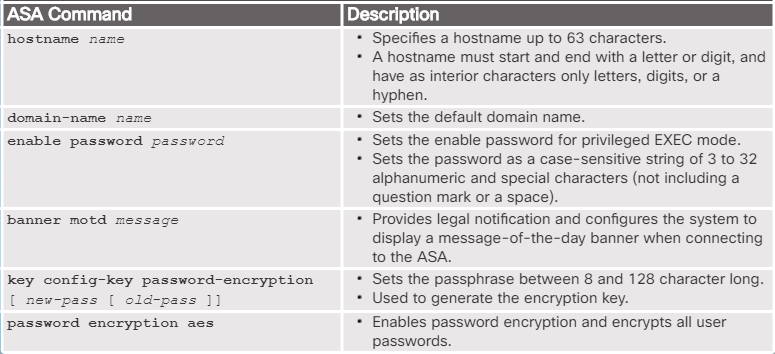
\includegraphics[scale=0.5]{pictures/ASAbasic.PNG}
\end{figure}

\subsection{Configuring Logical VLAN Interfaces}

When configuring an ASA 5505, there are two kinds of interfaces that need to be configured:

\begin{itemize}
\item Logical VLAN interfaces -- These interfaces are configured with the Layer 3 information including a name, security level, and IP address.
\item Physical switch ports -- These are Layer 2 switch ports which are assigned to the logical VLAN interfaces.
\end{itemize}

\begin{figure}[hbtp]
\caption{Logical VLAN interface command}\label{ASAlogicalVLAN}
\centering
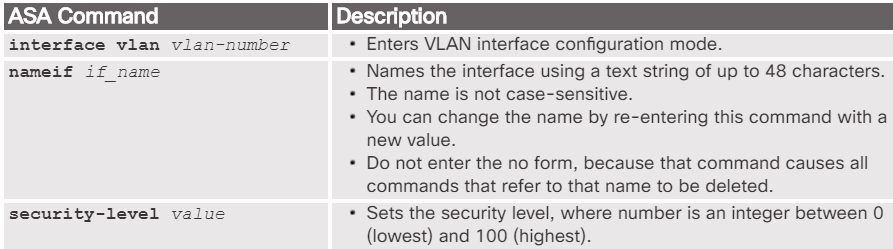
\includegraphics[scale=0.5]{pictures/ASAlogicalVLAN.PNG}
\end{figure}


An ASA 5505 with a Base license does not allow three fully functioning VLAN interfaces to be created. However, a third  \emph{limited} VLAN interface can be created if it is first configured with the \code{no forward interface vlan <num>} command (figure \ref{ASAlogicalVLAN}). This command limits the interface from initiating contact with another VLAN. Therefore, when the inside and outside VLAN interfaces are configured, the no forward interface vlan number command must be entered before the \code{nameif} command is entered on the third interface. The \code{<num>} argument specifies the VLAN ID to which this VLAN interface cannot initiate traffic. The Security Plus license is required to achieve full functionality.\\

\subsection{Static routes and IP addresses}

Switch ports on the same VLAN can communicate with each other using hardware switching. But when a switch port on VLAN 1 wants to communicate with a switch port on VLAN 2, then the ASA applies the security policy to the traffic and routes between the two VLANs. If an ASA is configured as a DHCP client, then it can receive and install a default route from the upstream device. Otherwise, a default static route must be configured using the \code{route <ifname> 0.0.0.0 0.0.0.0 next-hop-ip-address} command. To verify the route entry, use the \code{show route} command.\\

The IP address of an interface can be configured using one of the following options: DHCP, PPPoE, or manually. The table in Figure \ref{SVIaddr} lists the commands to configure an IP address on an interface. 

\begin{figure}[hbtp]
\caption{Configure IP addresses on logical VLAN interfaces}\label{SVIaddr}
\centering
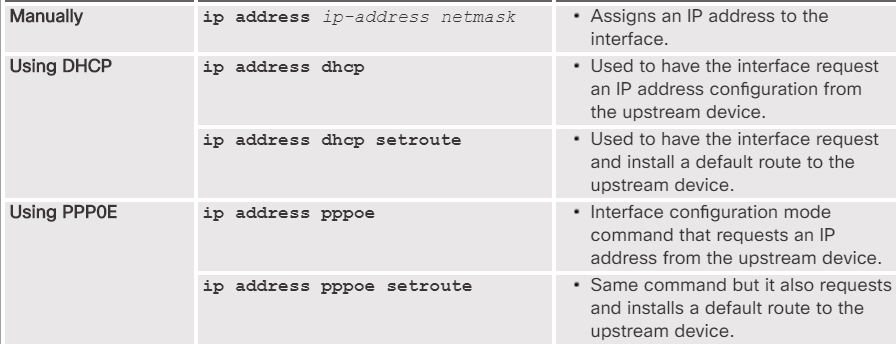
\includegraphics[scale=0.5]{pictures/SVIaddr.PNG}
\end{figure}

\subsection{Remote access}

\begin{figure}[hbtp]
\caption{ASA Telnet configuration commands}\label{TelnetConfigASA}
\centering
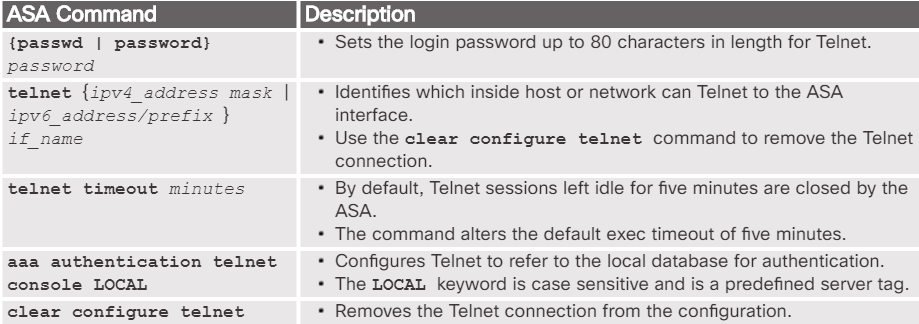
\includegraphics[scale=0.5]{pictures/TelnetConfigASA.PNG}
\end{figure}

\begin{figure}[hbtp]
\caption{Sample ASA Telnet configuration}\label{TelnetExample}
\centering
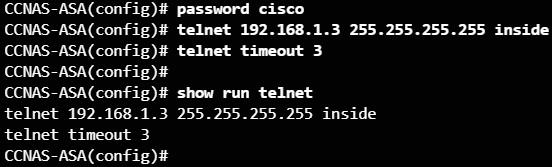
\includegraphics[scale=0.5]{pictures/TelnetExample.PNG}
\end{figure}


\begin{figure}[hbtp]
\caption{ASA ssh configuraiton commands}\label{SSHconfigASA}
\centering
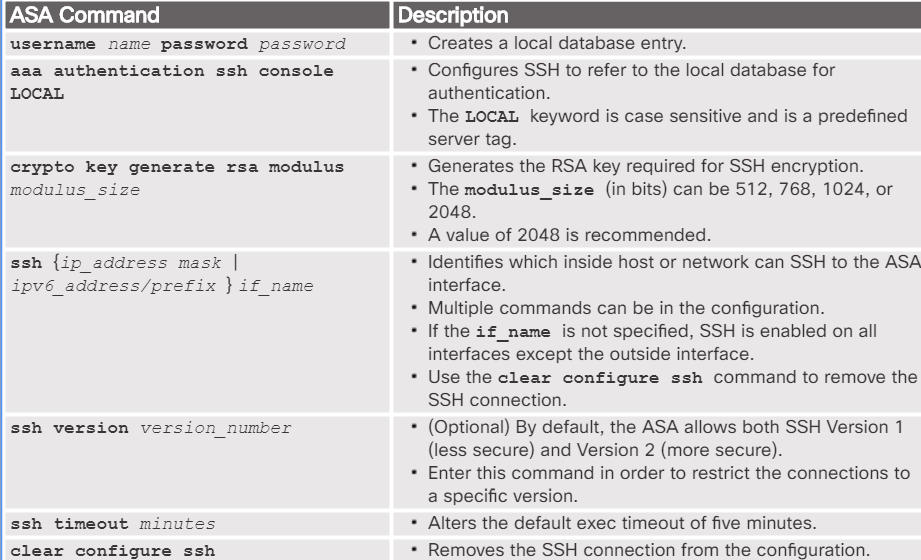
\includegraphics[scale=0.5]{pictures/SSHconfigASA.PNG}
\end{figure}

\subsection{NTP configuration}

\begin{figure}[hbtp]
\caption{NTP authentication commands}
\centering
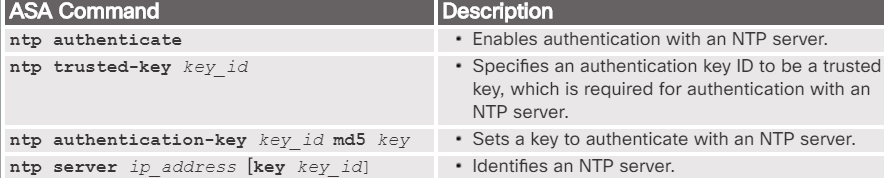
\includegraphics[scale=0.5]{pictures/NTPauthentication.PNG}
\end{figure}

\subsection{DHCP configuration}

\begin{figure}[hbtp]
\caption{DHCP server commands}\label{DHCPcommandList}
\centering
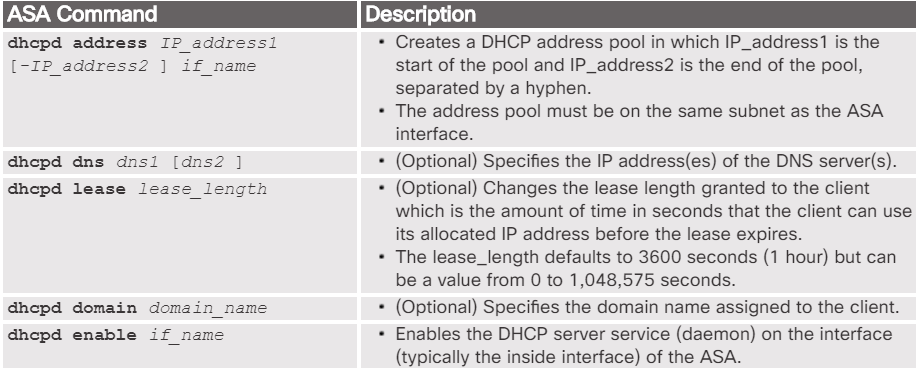
\includegraphics[scale=0.5]{pictures/DHCPcommandList.PNG}
\end{figure}


The example in Figure \ref{DHCPcommand} enables the DHCP service for inside clients on an ASA 5505. The ASA 5505 Base license can provide IP configuration information for up to 32 DHCP clients. If the ASA outside interface was configured as a DHCP client, then the \code{dhcpd auto outside} global configuration mode command can be used to pass the DHCP-obtained information to the DHCP inside clients.

\begin{figure}[hbtp]
\caption{Sample configuration ASA as an DHCP server}\label{DHCPcommand}
\centering
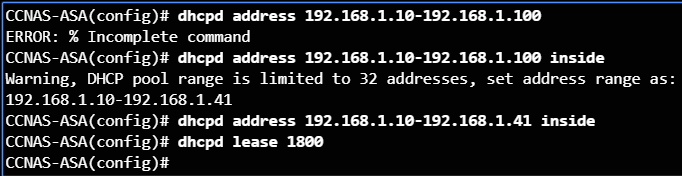
\includegraphics[scale=0.5]{pictures/DHCPcommand.PNG}
\end{figure}

\section{Objects and Object Groups}

The ASA supports objects and object groups. An object can be a particular IP address, an entire subnet, a range of addresses, a protocol, or a specific port or range of ports. The object can then be re-used in several configurations. The advantage is that when an object is modified, the change is automatically applied to all rules that use the specified object. There are two types of objects that can be configured:

\begin{itemize}
\item Network object -- Contains a single IP address and subnet mask. Network objects can be of three types: host, subnet, or range. 
\item Service object -- Contains a protocol and optional source and/or destination port.
\end{itemize}

To create a network object, use the \code{object network <name>} global configuration mode command. The prompt changes to network object configuration mode. A network object name can contain only one IP address and mask pair. Therefore, there can only be one statement in the network object. Entering a second IP address/mask pair replaces the existing configuration (figure \ref{NetObject}).

\begin{figure}[hbtp]
\caption{Network object configuration}\label{NetObject}
\centering
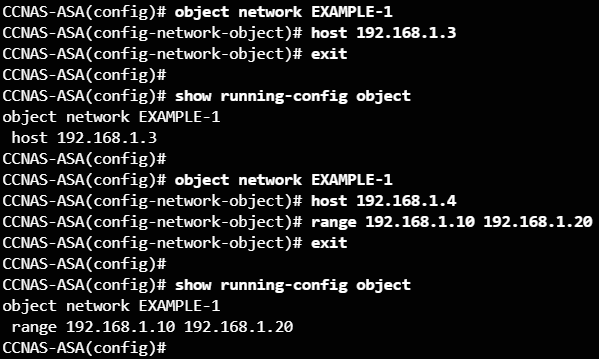
\includegraphics[scale=0.5]{pictures/NetObject.PNG}
\end{figure}

To create a service object, use the object service object-name global configuration mode command. The prompt changes to service object configuration mode. The service object can contain a protocol, ICMP, ICMPv6, TCP, or UDP port (or port ranges).

\begin{figure}[hbtp]
\caption{Service object configuration}\label{ServObject}
\centering
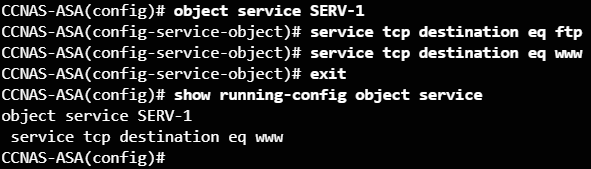
\includegraphics[scale=0.5]{pictures/ServObject.PNG}
\end{figure}

Objects can be grouped together to create an object group. By grouping like objects together, an object group can be used in an access control entry (ACE) instead of having to enter an ACE for each object separately.

\begin{figure}[hbtp]
\caption{Create a network object group}\label{NetObjGrp}
\centering
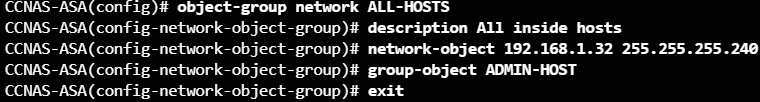
\includegraphics[scale=0.7]{pictures/NetObjGrp.PNG}
\end{figure}

To configure a network object group, use the \code{object-group network <name>} global configuration mode command. After entering the command, add network objects to the network group using the \code{network-object} and \code{group-object} commands (figure \ref{NetObjGrp}). \textbf{Note:} A network object group cannot be used to implement NAT. A network object is required to implement NAT.\\

\begin{figure}[hbtp]
\caption{ICMP-type object group}\label{ICMPobjgrp}
\centering
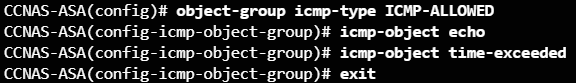
\includegraphics[scale=0.5]{pictures/ICMPobjgrp.PNG}
\end{figure}


To configure an ICMP object group, use the object-group icmp-type grp-name global configuration mode command (figure \ref{ICMPobjgrp}). After entering the command, add ICMP objects to the ICMP object group using the icmp-object and group-object commands.\\

\section{Restricting traffic with ACL}

To allow connectivity between interfaces with the same security levels, the \code{same-security-traffic permit inter-interface} global configuration mode command is required. To enable traffic to enter and exit the same interface, such as when encrypted traffic enters an interface and is then routed out the same interface unencrypted, use the \code{same-security-traffic permit intra-interface} global configuration mode command.\\

\begin{figure}[hbtp]
\caption{ACL configuration without Object groups}\label{withoutObj}
\centering
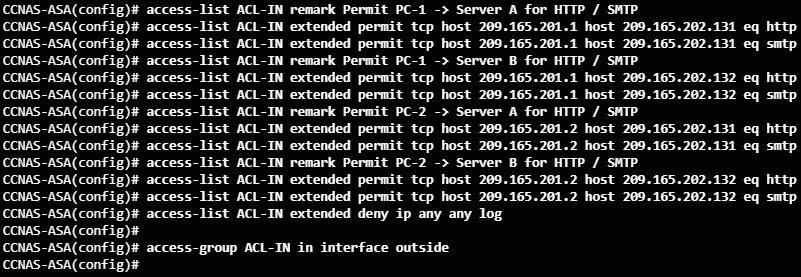
\includegraphics[scale=0.7]{pictures/withoutObj.PNG}
\end{figure}

Object grouping is a way to group similar items together to reduce the number of ACEs (comparing figure \ref{withoutObj} and \ref{withObj}). By grouping like objects together, object groups can be used in an ACL instead of having to enter an ACE for each object separately. 

\begin{figure}[hbtp]
\caption{ACL configuration using Network object group}\label{withObj}
\centering
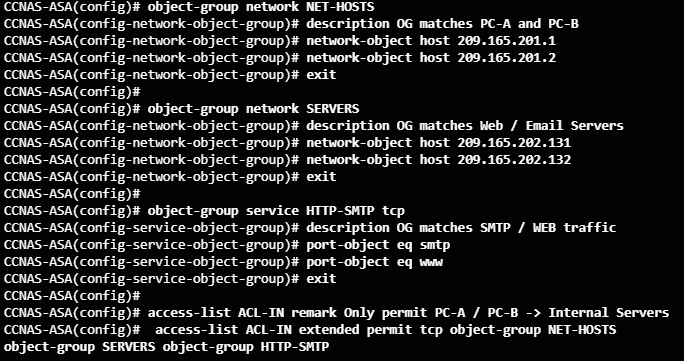
\includegraphics[scale=0.7]{pictures/withObj.PNG}
\end{figure}

\section{NAT configuration in ASA}

Use the \code{show xlate} and \code{show nat} detail commands to verify translations, as shown in Figure 4. It may be necessary to use the \code{clear nat counters} command when testing NAT.

\subsection{Static NAT}

Static NAT is configured when a single inside address is mapped to only one outside address. For instance, static NAT can be used when a server must be accessible from the outside.

\subsection{Dynamic NAT}

In figure \ref{DynamicNAT}, the inside hosts on the 192.168.1.0/27 network will be dynamically assigned a range of public IP address from 209.165.200.240 to 209.165.200.248. The PUBLIC network object identifies the public IP addresses to be translated to while the DYNAMIC-NAT identifies the internal addresses to be translated. The name \code{inside} is the interface connected to the private network, while \code{outside} interface connected to the Internet.\\

\begin{figure}[hbtp]
\caption{Dynamic NAT configuration on ASA}\label{DynamicNAT}
\centering
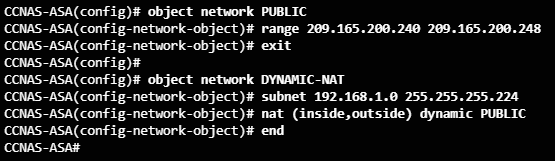
\includegraphics[scale=0.7]{pictures/DynamicNAT.PNG}
\end{figure}

Figure \ref{DynamicNATreturn} displays the configuration to allow return ICMP traffic from outside hosts.

\begin{figure}[hbtp]
\caption{Enable return traffic}\label{DynamicNATreturn}
\centering
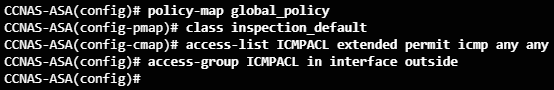
\includegraphics[scale=0.7]{pictures/DynamicNATreturn.PNG}
\end{figure}

After the inside host pings the outside host, verify the network address translation using the \code{show xlate} command. Additional information can be gathered using the \code{show nat} and \code{show nat detail} commands.

\subsection{PAT}

Only one network object is required when overloading the outside interface (figure \ref{PAT}). To enable inside hosts to overload the outside address, use the commands in figure 

\begin{figure}[hbtp]
\caption{PAT configuration in ASA}\label{PAT}
\centering
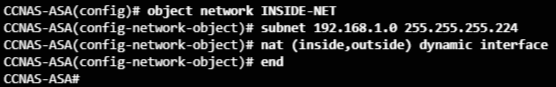
\includegraphics[scale=0.7]{pictures/PAT.PNG}
\end{figure}

\section{AAA in ASA}

To configure a TACACS+ or RADIUS server, use the commands listed in Figure \ref{sampleTACASasa}. To erase all AAA server configurations, use the \code{clear config aaa-server} command. To view all user accounts, use the \code{show running-config aaa-server} command.\\

\begin{figure}[hbtp]
\caption{Sample TACAS+ configuraiton in ASA}\label{sampleTACASasa}
\centering
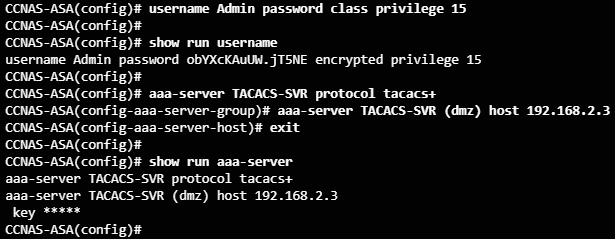
\includegraphics[scale=0.7]{pictures/sampleTACASasa.PNG}
\end{figure}


To authenticate users who access the ASA CLI over a console, SSH, HTTPS (ASDM), or Telnet connection, or to authenticate users who access privileged EXEC mode using the \code{enable} command, use \emph{ONE} of the\code{aaa authentication console} command in figure \ref{AAAconfigASA}.

\begin{figure}[hbtp]
\caption{Sample AAA configuration in ASA}\label{AAAconfigASA}
\centering
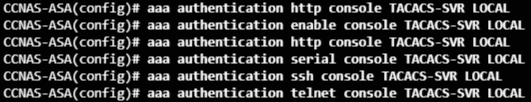
\includegraphics[scale=1]{pictures/AAAconfigASA.PNG}
\end{figure}


\section{Modular Policy Framework (MPF)}

A Modular Policy Framework (MPF) configuration defines a set of rules for applying firewall features, such as traffic inspection and QoS. MPF can be used for advanced Application Layer inspection of traffic by classifying at Layers 5 through 7. Cisco MPF uses these three configuration objects to define: Class map, Policy map, and Service policy. There are four steps to configure MPF on an ASA:

\begin{itemize}
\item Configure extended ACLs to identify granular traffic that can be specifically referenced in the class map. For example, ACLs can be used to match TCP traffic, UDP traffic, HTTP traffic, or all traffic to a specific server.

\item Configure the class map to identify traffic (figure \ref{classmap}.

\item Configure a policy map to apply actions to those class maps.

\item Configure a service policy to attach the policy map to an interface.
\end{itemize}

\begin{figure}[hbtp]
\caption{Configure the class map to identify traffic}\label{classmap}
\centering
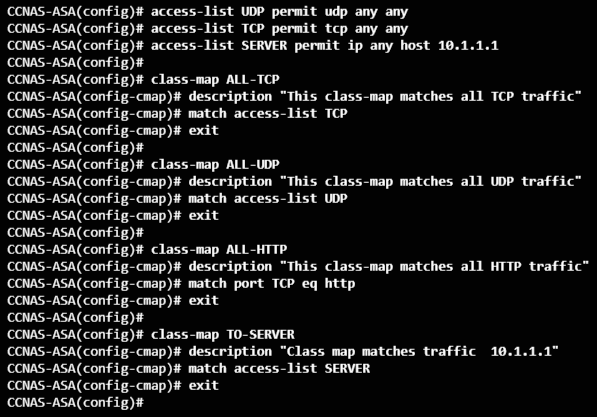
\includegraphics[scale=0.7]{pictures/classmap.PNG}
\end{figure}

\begin{figure}[hbtp]
\caption{Configure a policy map to apply actions to those class maps, and then create a service policy to attach the policy map to an interface}\label{MPFimplementation}
\centering
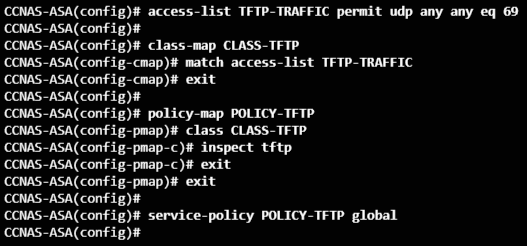
\includegraphics[scale=0.7]{pictures/MPFimplementation.PNG}
\end{figure}

